% Auto-generated by infra/generate_fault_chart.py — do not edit by hand.
% Source: documentation/report/e2e_runs/fault_injection/slots_timeline.csv
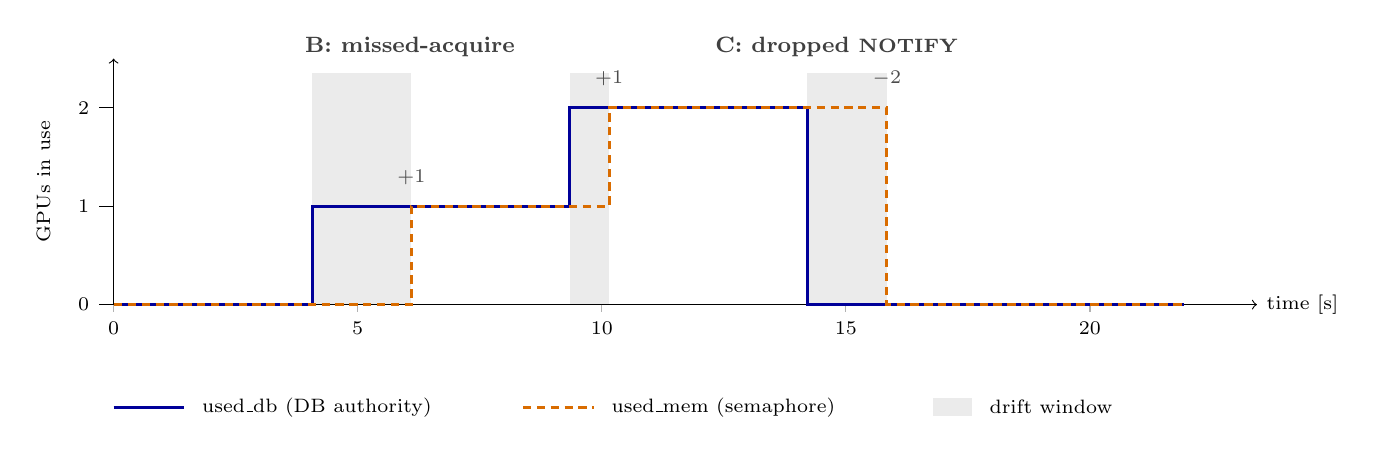
\begin{tikzpicture}[x=0.62cm, y=1.25cm, font=\footnotesize,
    dbline/.style={draw=blue!60!black, line width=1.1pt},
    memline/.style={draw=orange!85!black, line width=1.1pt, dash pattern=on 3pt off 2pt},
    driftband/.style={fill=black!8, draw=none},
    delta/.style={font=\scriptsize, text=black!70},
  ]
  \fill[driftband] (4.07,0) rectangle (6.10,2.35);
  \fill[driftband] (9.34,0) rectangle (10.15,2.35);
  \fill[driftband] (14.21,0) rectangle (15.84,2.35);
  \draw[->] (0,0) -- (23.42,0);
  \node[anchor=west, font=\scriptsize] at (23.42,0) {time [s]};
  \draw[->] (0,0) -- (0,2.5);
  \draw (0,0) -- (-0.3,0) node[anchor=east, font=\scriptsize] {0};
  \draw (0,1) -- (-0.3,1) node[anchor=east, font=\scriptsize] {1};
  \draw (0,2) -- (-0.3,2) node[anchor=east, font=\scriptsize] {2};
  \node[anchor=south, rotate=90, font=\scriptsize] at (-1.1,1.25) {GPUs in use};
  \draw[black!30] (0,0) -- (0,-0.08) node[anchor=north, font=\scriptsize, text=black] {0};
  \draw[black!30] (5,0) -- (5,-0.08) node[anchor=north, font=\scriptsize, text=black] {5};
  \draw[black!30] (10,0) -- (10,-0.08) node[anchor=north, font=\scriptsize, text=black] {10};
  \draw[black!30] (15,0) -- (15,-0.08) node[anchor=north, font=\scriptsize, text=black] {15};
  \draw[black!30] (20,0) -- (20,-0.08) node[anchor=north, font=\scriptsize, text=black] {20};
  \draw[dbline] (0.01,0) -- (4.07,0) -- (4.07,1) -- (9.34,1) -- (9.34,2) -- (14.21,2) -- (14.21,0) -- (21.92,0);
  \draw[memline] (0.01,0) -- (6.10,0) -- (6.10,1) -- (10.15,1) -- (10.15,2) -- (15.84,2) -- (15.84,0) -- (21.92,0);
  \node[delta, anchor=south] at (6.10,1.12) {$+1$};
  \node[delta, anchor=south] at (10.15,2.12) {$+1$};
  \node[delta, anchor=south] at (15.84,2.12) {$-2$};
  \node[font=\footnotesize\bfseries, text=black!75] at (6.07,2.62) {B: missed-acquire};
  \node[font=\footnotesize\bfseries, text=black!75] at (14.81,2.62) {C: dropped {\scriptsize NOTIFY}};
  \begin{scope}[shift={(0,-1.15)}, x=1cm, y=0.45cm]
    \draw[dbline] (0,0.3) -- (0.9,0.3);
    \node[anchor=west, font=\scriptsize] at (1.0,0.3) {used\_db (DB authority)};
    \draw[memline] (5.2,0.3) -- (6.1,0.3);
    \node[anchor=west, font=\scriptsize] at (6.2,0.3) {used\_mem (semaphore)};
    \fill[driftband] (10.4,0.05) rectangle (10.9,0.55);
    \node[anchor=west, font=\scriptsize] at (11.0,0.3) {drift window};
  \end{scope}
\end{tikzpicture}
